%====================================================================================================
% --------------------------------------------- Definite Integral -----------------------------------
\chapter{Určitý integrál}
\minitoc
\newpage  
\section{Motivace} 
  %----------------------------------
  % image: MAI_animated_integral.tex label: \label{MAI:fig_anim_int}
    % \documentclass{book}
% \usepackage{ifthen}
% \usepackage{tikz}
%   \usetikzlibrary{intersections}
%   \usetikzlibrary{calc}
% \usepackage{animate}

\newcounter{r}
\newcommand{\escalar}[1]{
\setcounter{r}{#1 * #1 * #1}
}
%
\newcounter{m}
\setcounter{m}{0}
\newcounter{mc}

% \begin{document}
    %\begin{frame}[fragile]{Animated Integral}
      %\centering
      \protect  % JAFA příkaz protect pomohl -> nemusí být \begin{frame}, který funguje divně (vysází se obsah
                % závorek, tj. [fragile]{Animated Integral})
        \begin{animateinline}[loop, poster = first, controls, palindrome]{2}
          \whiledo{\them < 21}{
            \begin{tikzpicture}[scale=1.25]
              \draw[red,thick,<->] (-1,1) parabola bend (0,0) (2.1,4.41)
                  node[below right] {$y=x^2$};
              \draw[loosely dotted] (-1,0) grid (4,4);
              %\path[use as bounding box] (-2,-1) rectangle (5,5);
              \draw[->] (-0.2,0) -- (4.25,0) node[right] {$x$};
              \draw[->] (0,-0.25) -- (0,4.25) node[above] {$y$};
              \foreach \x/\xtext in {1/1, 2/2, 3/3}
                \draw[shift={(\x,0)}] (0pt,2pt) -- (0pt,-2pt) node[below] {$\xtext$};
              \foreach \y/\ytext in {1/1, 2/2, 3/3, 4/4}
                \draw[shift={(0,\y)}] (2pt,0pt) -- (-2pt,0pt) node[left] {$\ytext$};
              %
              \setcounter{mc}{\value{m}*\value{m}}
              \shade[top color=blue,bottom color=gray!50]
                  (0,0) parabola (0.1*\them,0.01*\themc) |- (0,0);
              \escalar{\them}
              \draw (3cm,2pt) node[above]
                {$\displaystyle\int\limits_0^{\them/10}\!\!x^2\mathrm{d}x=\displaystyle\frac{\ther}{3000}$};
              \draw[fill=orange,color=orange] (0.1*\them,0.01*\themc) circle (0.5pt);
            \end{tikzpicture}
            %
            \stepcounter{m}
            \ifthenelse{\them < 21}{
                    \newframe
            }{
                \end{animateinline}\relax % BREAK
            }
          } % END \whiledo...
      \label{MAI:fig_anim_int}
    %\end{frame} 
  
% \end{document}  
  %---------------------------------- 

\subsection{Výpočet integrálu}
    \begin{example}Metodou per partes spočítejte integrály:$\displaystyle\int_1^{ln5}{(x+1)e^xdx}$
      \begin{align*}
        \int{(x+1)e^xdx} &= \int{e^xdx}+\int{x\cdot e^xdx} \\
                         &= e^x + (x-1)e^x = xe^x \\
        \int_1^{ln5}{(x+1)e^xdx} &= [xe^x]_1^{ln5} = 5ln5-e\\
      \end{align*}
      kde integrál
      \begin{equation*}
          \int{xe^xdx}=
            \left[\begin{array}{cc}
              u=x   & dv=e^x \\
              du=dx & v=e^x
            \end{array}\right]=
            xe^x-\int{e^xdx} = xe^x - e^x+C
      \end{equation*}
    \end{example}

\newpage
\section{Vlastnosti určitého integrálu}
  V této kapitole mluvíme o spojitých funkcích $\Rightarrow$ příslušné integrály tedy vždy
  existují. Čerpáno z knih:
  \cite{Knichal}.

  \begin{lemma}
    \textbf{První věta o střední hodnotě integrálního počtu}: Je-li funkce $f(x)$ spojitá v
    intervalu $\langle a, b\rangle$, existuje alespoň jeden takový bod $c\in(a, b)$, že platí

    \begin{equation}\label{MA:eq_av1}
      \int_a^b f(x)dx = (b-a)f(c).
    \end{equation}
  \end{lemma}

  \begin{proof} Použitím Lagrangeovy věty napsané pro funkci $F(x)$, primitivní na intervalu
    $\langle a, b\rangle$ k dané funkci $f(x)$. Podmínky věty jsou zřejmě splněny: $F(x)$ je
    spojitá na intervalu $\langle a, b\rangle$ a má všude derivaci $F'(x)= f(x)$. Tedy existuje
    alespoň jeden bod $c\in(a, b)$,
    
      %----------------------------------
        % image: MAI_rolle_02.tex label: \label{MA:fig_rolle_02} 
        % \documentclass{article}
% \usepackage{tikz}
% \usetikzlibrary{decorations.markings}
% \usetikzlibrary{intersections}
% \usepackage{wrapfig}                   % Floats, Figures and Captions  
% \usetikzlibrary{calc}

% \begin{document}
 
    \begin{figure}[hb!]
        \centering
        \begin{tikzpicture}
           [scale=3,line cap=round,
            % Styles
              axes/.style=,
              important line/.style={very thick},
              information text/.style={rounded corners,fill=red!10,inner sep=1ex}]
          \begin{scope}[axes]     
            \draw[->] (-0.2, 0) -- (1.5, 0) node[right] {$x$} coordinate(x axis);
            \draw[->] (0, -0.2) -- (0, 1.5) node[left] {$y$} coordinate(y axis);
          \end{scope}
          % my function  
           \draw[very thick,red](1.5,1.4) node[left=1pt,fill=white]{$y=f(x)$};
           \coordinate [label={[blue]left:$D$}] (D) at (0.3,0.5);
           \coordinate [label={[blue]right:$C$}] (C) at (1.2,1.2);
           \draw[name path=func] (D) .. controls (1.0,0.5) and (0.5,1.2) .. (C);
          % horizontal line
           \draw[name path=my_line, gray, dotted] (0.75,0) node[below, red]{$c$} -- (0.75,0.9);
          % intersection between vertical line and my function
           \fill[red, opacity=0.5, name intersections={of=func and my_line, by={intersect}}]
                (intersect) circle (1pt);
          % x-axis labels
           \draw[gray, dotted, text = blue] (D) -- +(0,-0.5) 
              node [label={[xshift=-0.2cm, yshift=0.5mm]$A$},below] (A) {$a$};
           \draw[gray, dotted, text=blue] (C) -- +(0,-1.2)
              node [label={[xshift=0.2cm, yshift=0.5mm]$B$},below] (B) {$b$};
           \draw[red](-0.05,-0.08) node[left=1pt,fill=white]{$0$};
          % y-axis labels
           \draw[gray, dotted] let \p1=(D), \p2=(intersect), \p3=(C) in (\x1,\y2)
              -- +(-\x1,0) node[left, red]{$f(c)$} 
              -- (\x1,\y2) node[above, blue] (F) {$F$} 
              -- (\x3,\y2) node[right, blue]{$E$}; 
          % dotted line between F and D
           \draw[gray, dotted] (F) -- (D);
        \end{tikzpicture}
        \caption{ }\label{MAI:fig_rolle_02}
    \end{figure}
  
%\end{document}  
      %----------------------------------   
    
      že $$F(b)-F(a) = (b-a)F'(c),$$ čímž je věta dokázána, neboť $F(b)-F(a) = \int_a^bf(x)dx$ a
      $F'(c) = f(c)$. Funkční hodnotu $f(c)$, danou podle (\ref{MA:eq_av1}) rovnicí  
      \begin{equation}\label{MA:eq_av2}
         f(c) = \frac{1}{b-a}\int_a^b f(x)dx
      \end{equation}
      nazýváme \texttt{střední hodnotou}.
  \end{proof}

  Pro spojitou nezápornou funkci $f(x)$, lze větu o střední hodnotě jednoduše geometricky
  interpretovat dle (obr.\ref{MAI:fig_rolle_02}). Levá strana (\ref{MA:eq_av1}) určuje obsah
  křivočarého lichoběžníka $ABCD$, pravá strana obsah obdélníka $ABEF$. Podle této věty nabývá
  funkce $f(x)$ aspoň v jednom bodě intervalu $(a, b)$ takové hodnoty $f(c)$, že uvažovaný
  křivočarý lichoběžník má stejný obsah jako obdélník o základně $b-a$ a výšce $f(c)$ (str. 155
  knihy \cite{Knichal}).

  \begin{example} Určete střední hodnotu $i_s$ střídavého proudu $$i(t) = I_0\sin\omega t$$ v
    časovém intervalu $\langle 0, \frac{T}{2}\rangle$ (v průběhu jedné poloviny periody). $I_0$ je
    maximální hodnota proudu (obr. \ref{MA:fig_Iav_exam}), perioda $T$ je dána vztahem $T =
    \frac{2\pi}{\omega}$
    %----------------------------------
      % image: MAI_rolle_02.tex label: \label{MA:fig_Iav_exam}
      % \documentclass{article}
% \usepackage{tikz}
% \usetikzlibrary{decorations.markings}
% \usetikzlibrary{intersections}
% \usetikzlibrary{calc}

% \begin{document}
 
      {\centering
       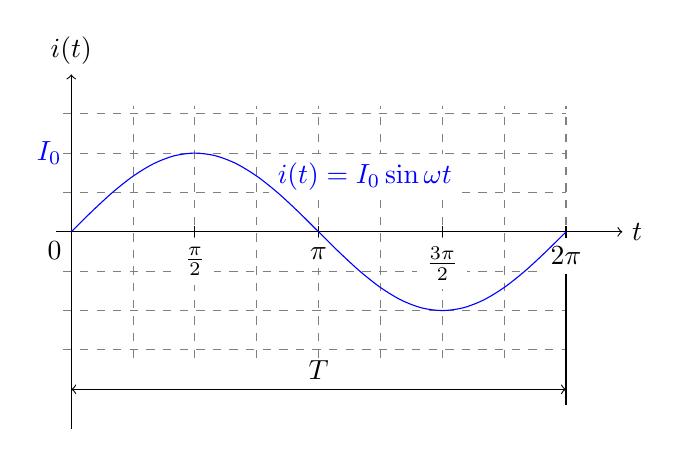
\begin{tikzpicture}[domain=0:2*pi] 
         \draw[xstep=pi/4, ystep=0.5, dashed, color=gray] (-0.1,-1.6) grid (2*pi,1.6); 
         \draw[->] (-0.2,0) -- (7,0) node[right] {$t$}; 
         \draw[->] (0,-2.5) -- (0,2) node[above] {$i(t)$}; 
         % text 
         \node[below left](0,0){$0$};
         \node[left, color=blue] at (0,1.0) {$I_0$}; 
         % period
         \draw[<->] (0,-2) -- (pi,-2) node[above]{$T$} --(2*pi,-2);
         \draw (2*pi,-2.2) -- (2*pi,0); 
         \foreach \x/\xtext in {0.5*pi/\frac{\pi}{2} ,pi/\pi, 1.5*pi/\frac{3\pi}{2}, 2*pi/2\pi}
         \draw[shift={(\x,0)}] (0pt,2pt) -- (0pt,-2pt) node[below, fill=white] {$\xtext$};  
         \node[below right, color=blue, fill=white] at (2.5,1.0) {$i(t) = I_0\sin\omega t$};
         % function 
         \draw[color=blue, smooth]   plot (\x,{sin(\x r)}); 
       \end{tikzpicture}  
       \captionsetup{type=figure}   
       \captionof{figure}{}\label{MA:fig_Iav_exam}
    \par}
  
%\end{document}  
    %----------------------------------

    Podle \ref{MA:eq_av2} bude
    \begin{align*}
     i_s &=  \frac{2}{T}
             \int_0^{\frac{T}{2}}I_0\sin\omega t\dd{t} =
             \frac{2I_0}{T}\left[-\frac{\cos\omega t}{\omega}\right]_0^{\frac{T}{2}}        \\
         &=  \frac{2I_0}{T}\frac{1}{\omega}\left(-\cos\frac{\omega T}{2}+ \cos 0\right)     \\
         &=  \frac{2I_0}{2\pi}(-\cos\pi + \cos 0) = \frac{2}{\pi}I_0 \doteq 0,637 I_0.
  \end{align*}

  Tato hodnota se rovná intenzitě elektrického proudu, při kterém by vodičem v průběhu uvažované
  poloviny periody prošel stejný elektrický náboj jako při proudu střídavém.
  \end{example}

  \begin{example} Efektivní hodnota $i_{ef}$ střídavého proudu $$i(t) = I_0\sin\omega t$$ (viz
    předchozí příklad) je definována jako odmocnina ze střední hodnoty funkce $i^2(t)$ v průběhu
    jedné periody $T = \frac{2\pi}{\omega}$. Tedy
    \begin{align*}
      i_{ef}^2 &= \frac{1}{T}\int_0^T I_0^2\sin^2\omega t\dd{t} = 
                  \frac{1}{T}\int_0^T \frac{I_0^2}{2}(1- \cos2\omega t)\dd{t}           \\
               &= \frac{I_0^2}{2T}
                  \left[
                    t-\frac{\sin2\omega t}{2\omega}
                  \right]_0^T = \frac{I_0^2}{2}
    \end{align*}
    neboť $\sin2\omega T=\sin4\pi = 0.$ Odtud $$i_{ef} = \frac{I_0}{\sqrt{2}}.$$ Střídavý proud
    $i(t) = I_0\sin\omega t$ má na témže odporu stejný výkon jako stejnosměrný proud o intenzitě
    $i = 0,707I_0$.
  \end{example}
  Následující věta může být využita k odhadu některých integrálů
  \begin{lemma}
    \textbf{Druhá věta o střední hodnotě integrálního počtu}: Jsou-li funkce $f(x)$ a $g(x)$
    spojité v intervalu $\langle a, b \rangle$ a je-li funkce $g(x)$ v $\langle a, b \rangle$
    nezáporná a nerostoucí, existuje alespoň jeden bod $c\in\langle a, b \rangle$ tak, že platí
    \begin{equation}\label{MA_eq_av3}
        \int_a^b f(x)g(x) = g(a)\int_a^c f(x)dx.
    \end{equation}
  \end{lemma}
  Zcela obdobnou větu lze vyslovit pro případ, že $g(x)$ je v intervalu $\langle a, b \rangle$
  nezáporná a neklesající, tj. na pravé straně \ref{MA_eq_av3} je pak integrál $g(b)\int_c^b
  f(x)dx$

  \begin{example} Odhadněte hodnotu integrálu
    \begin{equation}\label{MA_eq_sinx_x}
        \int_{100\pi}^{1000\pi}\frac{\sin x}{x}dx
    \end{equation}
    Řešení: Funkce $f(x) = \sin x$ a $g(x) = \frac{1}{x}$ jsou v uvažovaném intervalu $\langle
    100\pi, 1000\pi \rangle$ spojité a funkce $g(x)$ je kladná a nerostoucí.
    \begin{equation*}
      \int_{100\pi}^{1000\pi}\frac{\sin x}{x}dx = 
      \frac{1}{100\pi}\int_{100\pi}^c\sin xdx =\frac{1}{100\pi}\left(\cos100\pi - \cos c\right)
    \end{equation*}
    kde $c$ je kladné číslo z intervalu $\langle 100\pi, 1000\pi \rangle$. Dále pro všechna
    $c\in\langle 100\pi, 1000\pi \rangle$ platí $0\leq1-\cos c\leq2$, takže
    \begin{equation*}
        0\leq\int_{100\pi}^{1000\pi}\frac{\sin x}{x}dx\leq \frac{1}{50\pi}.
    \end{equation*}
  \end{example}   
%---------------------------------------------------------------------------------------------------
\printbibliography[heading=subbibliography]
\addcontentsline{toc}{section}{Seznam literatury}